\documentclass[a4paper,10pt]{article}
\usepackage[spanish]{babel}
\usepackage[utf8]{inputenc}
\usepackage[breaklinks=true]{hyperref}
\usepackage{verbatim}
\usepackage{amsmath}
\usepackage{graphicx}
\usepackage{subfig}
%\usepackage{subfigure}
\RequirePackage{fontawesome}
%opening

\begin{document}

\begin{titlepage}
\centering
{
\includegraphics[width=0.9\textwidth]{fing_uncuyo}\par}
\vspace{1cm}
{\bfseries\LARGE Universidad Nacional de Cuyo \par}
\vspace{1cm}
{\scshape\Large Facultad de Ingeniería \par}
\vspace{3cm}
{\scshape\Huge Predicción de Precios de Criptomonedas con ARIMA y Prophet \par}
\vspace{3cm}
{\itshape\Large Proyecto Final: Anexo II\\Inteligencia Artificial I \par}
\vfill
{\Large MOLINA, Mauro \par}
{\Large FLORES, Daniel Emiliano \par}
\vfill
{\Large Marzo 2022 \par}
\end{titlepage}

\newpage

\section{Gráficos de periodo mensual y semanal aleatorios con ARIMA(2,1,1)}

\begin{figure}
 \centering
  \subfloat[]{
   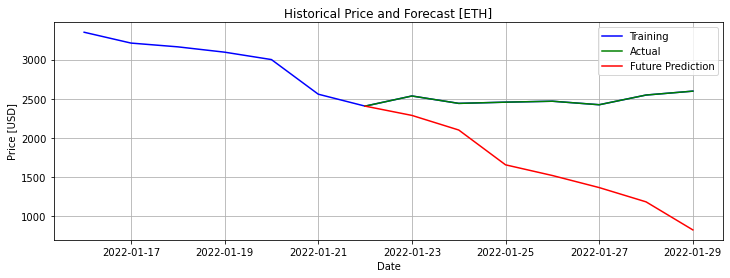
\includegraphics[width=0.5\textwidth]{./plots/arima/plots_eth_random_weekly/eth_wk1}}
  \subfloat[]{
   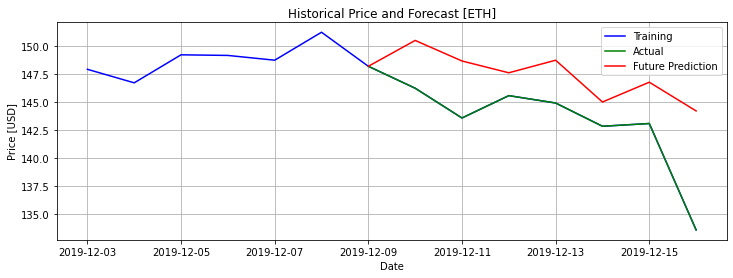
\includegraphics[width=0.5\textwidth]{./plots/arima/plots_eth_random_weekly/eth_wk2}} \\
  \subfloat[]{
   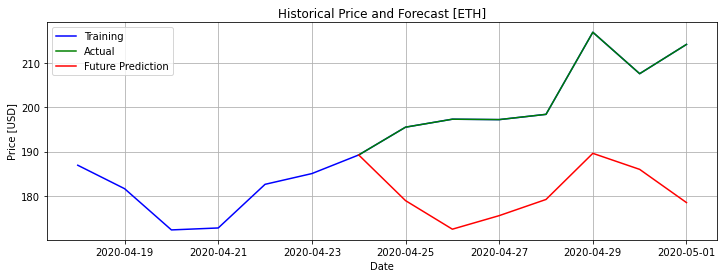
\includegraphics[width=0.5\textwidth]{./plots/arima/plots_eth_random_weekly/eth_wk3}}
   \subfloat[]{
   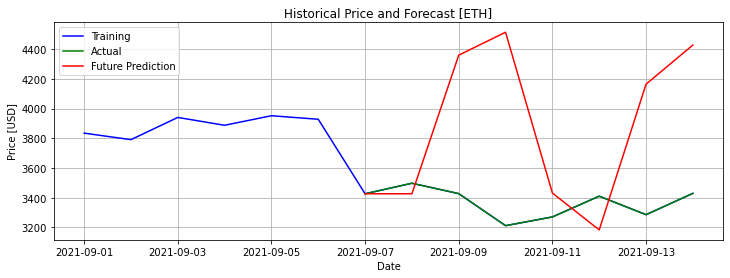
\includegraphics[width=0.5\textwidth]{./plots/arima/plots_eth_random_weekly/eth_wk4}} \\
   \subfloat[]{
   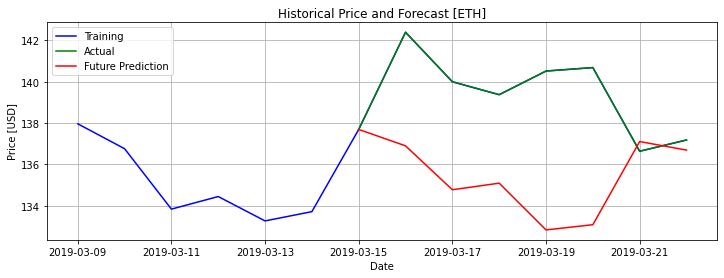
\includegraphics[width=0.5\textwidth]{./plots/arima/plots_eth_random_weekly/eth_wk5}}
   \subfloat[]{
   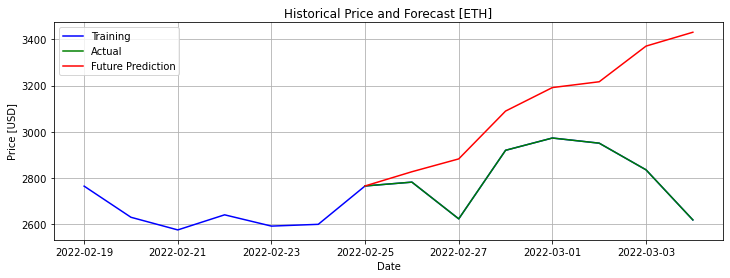
\includegraphics[width=0.5\textwidth]{./plots/arima/plots_eth_random_weekly/eth_wk6}} \\
   \subfloat[]{
   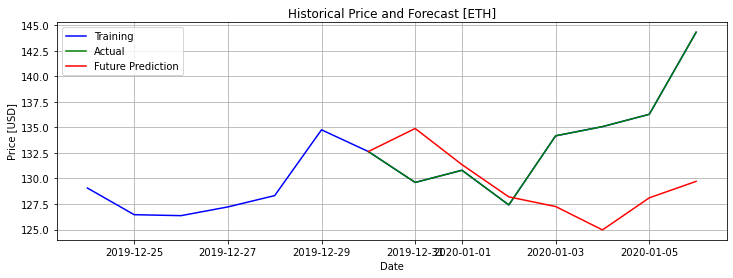
\includegraphics[width=0.5\textwidth]{./plots/arima/plots_eth_random_weekly/eth_wk7}}
   \subfloat[]{
   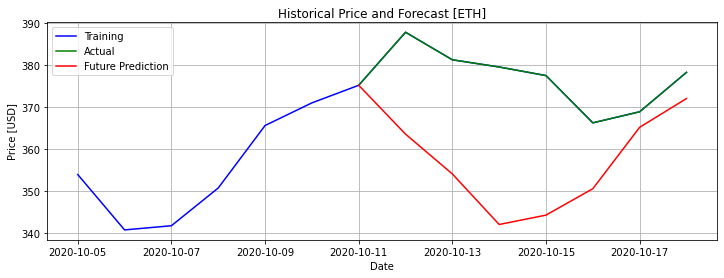
\includegraphics[width=0.5\textwidth]{./plots/arima/plots_eth_random_weekly/eth_wk8}} \\
   \subfloat[]{
   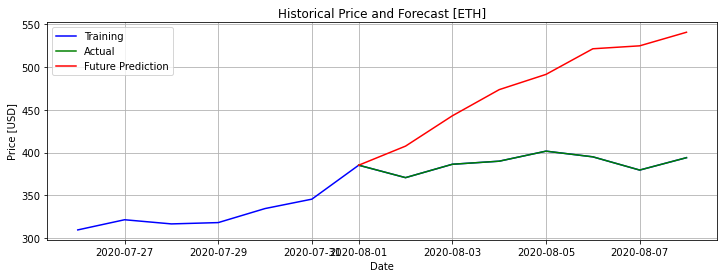
\includegraphics[width=0.5\textwidth]{./plots/arima/plots_eth_random_weekly/eth_wk9}}
   \subfloat[]{
   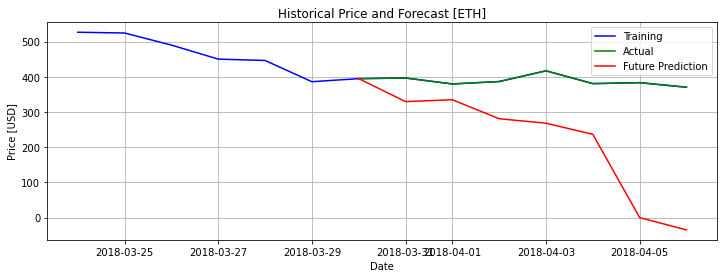
\includegraphics[width=0.5\textwidth]{./plots/arima/plots_eth_random_weekly/eth_wk10}}
  \caption{Predicción del modelo entrenado con 10 semanas aleatorias de ETH}
  \label{f:eth_wk_arima}
\end{figure}

\begin{table}[t]
 \begin{center}
  \begin{tabular}{|r|c|c|c|c|c|c|c|c|c|c|}
    Métrica & (a) & (b) & (c) & (d) & (e) & (f) & (g) & (h) & (i) & (j) \\ \hline
    MAE &  &  &  &  &  &  &  &  &  &  \\
    RMSE &  &  &  &  &  &  &  &  &  & \\
    sMAPE &  &  &  &  &  &  &  &  &  & \\ \hline
  \end{tabular}
  \caption{Fruta disponible}
  \label{tab:eth}
 \end{center}
\end{table}

\begin{figure}
 \centering
  \subfloat[]{
   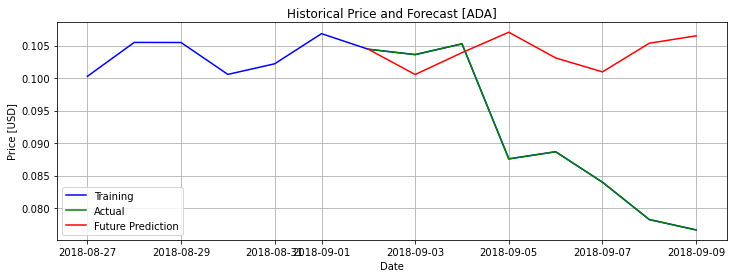
\includegraphics[width=0.5\textwidth]{./plots/arima/plots_ada_random_weekly/ada_wk1}}
  \subfloat[]{
   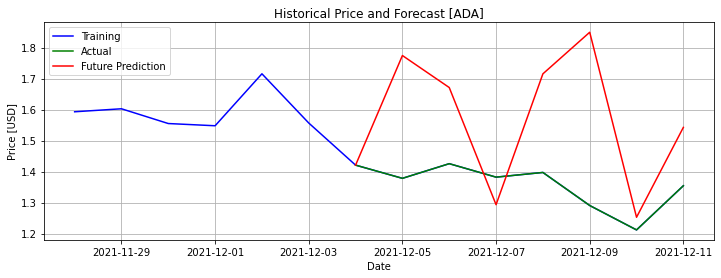
\includegraphics[width=0.5\textwidth]{./plots/arima/plots_ada_random_weekly/ada_wk2}} \\
  \subfloat[]{
   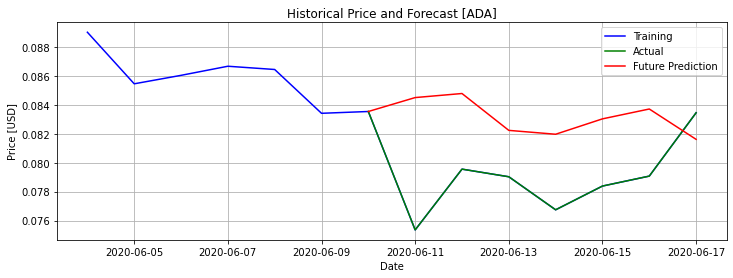
\includegraphics[width=0.5\textwidth]{./plots/arima/plots_ada_random_weekly/ada_wk3}}
   \subfloat[]{
   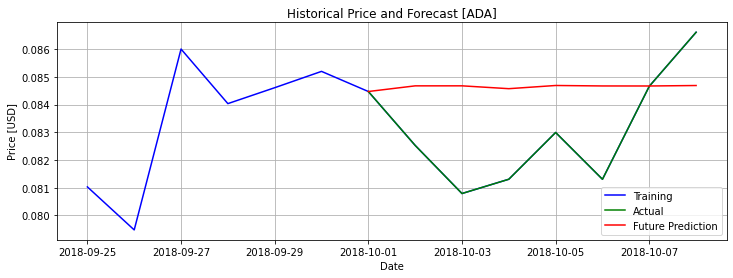
\includegraphics[width=0.5\textwidth]{./plots/arima/plots_ada_random_weekly/ada_wk4}} \\
   \subfloat[]{
   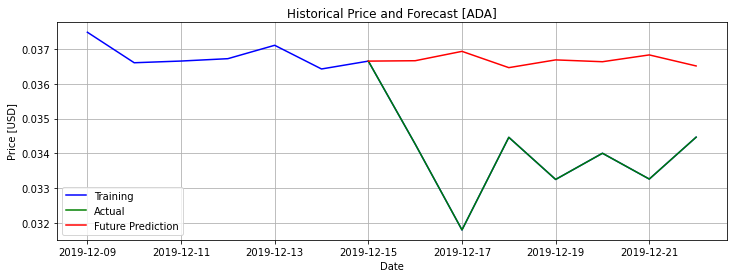
\includegraphics[width=0.5\textwidth]{./plots/arima/plots_ada_random_weekly/ada_wk5}}
   \subfloat[]{
   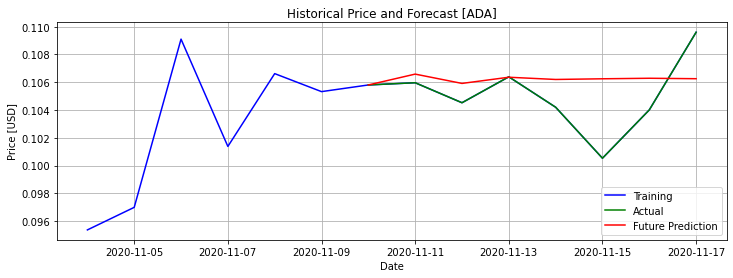
\includegraphics[width=0.5\textwidth]{./plots/arima/plots_ada_random_weekly/ada_wk6}} \\
   \subfloat[]{
   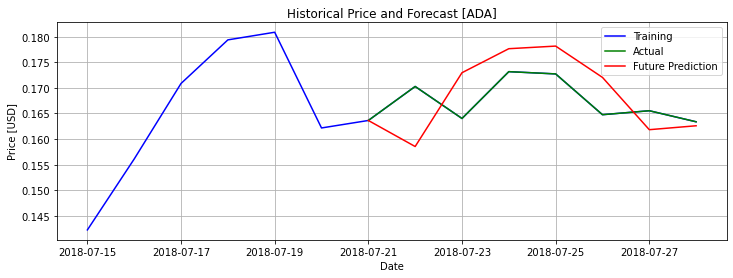
\includegraphics[width=0.5\textwidth]{./plots/arima/plots_ada_random_weekly/ada_wk7}}
   \subfloat[]{
   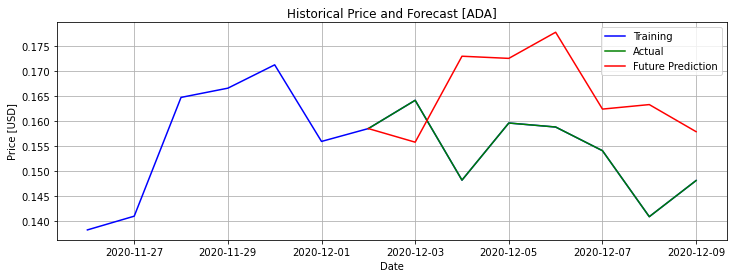
\includegraphics[width=0.5\textwidth]{./plots/arima/plots_ada_random_weekly/ada_wk8}} \\
   \subfloat[]{
   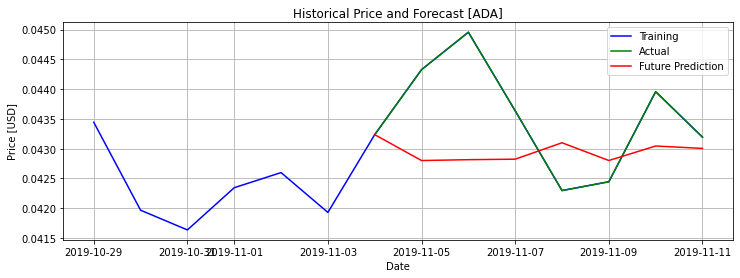
\includegraphics[width=0.5\textwidth]{./plots/arima/plots_ada_random_weekly/ada_wk9}}
   \subfloat[]{
   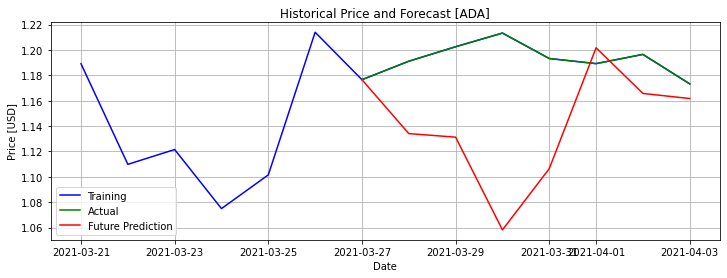
\includegraphics[width=0.5\textwidth]{./plots/arima/plots_ada_random_weekly/ada_wk10}}
  \caption{Predicción del modelo entrenado con 10 semanas aleatorias de ADA}
  \label{f:ada_wk_arima}
\end{figure}

\begin{table}[t]
 \begin{center}
  \begin{tabular}{|r|c|c|c|c|c|c|c|c|c|c|}
    Métrica & (a) & (b) & (c) & (d) & (e) & (f) & (g) & (h) & (i) & (j) \\ \hline
    MAE &  &  &  &  &  &  &  &  &  &  \\
    RMSE &  &  &  &  &  &  &  &  &  & \\
    sMAPE &  &  &  &  &  &  &  &  &  & \\ \hline
  \end{tabular}
  \caption{Fruta disponible}
  \label{tab:ada}
 \end{center}
\end{table}

\begin{figure}
 \centering
  \subfloat[]{
   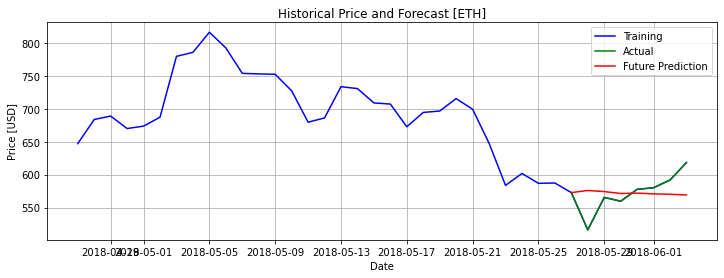
\includegraphics[width=0.5\textwidth]{./plots/arima/plots_eth_random_monthly/eth_mth1}}
  \subfloat[]{
   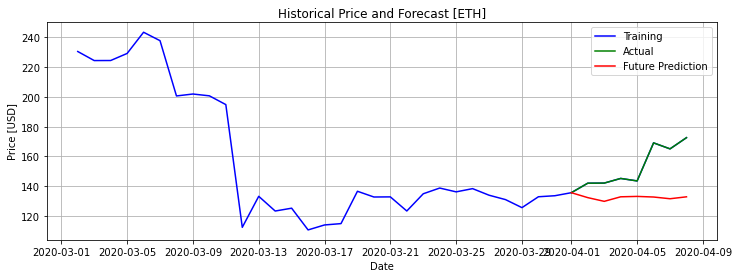
\includegraphics[width=0.5\textwidth]{./plots/arima/plots_eth_random_monthly/eth_mth2}} \\
  \subfloat[]{
   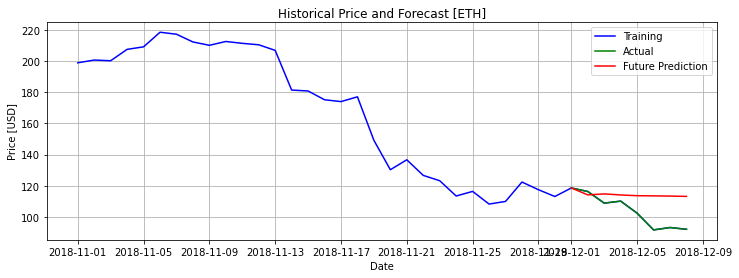
\includegraphics[width=0.5\textwidth]{./plots/arima/plots_eth_random_monthly/eth_mth3}}
   \subfloat[]{
   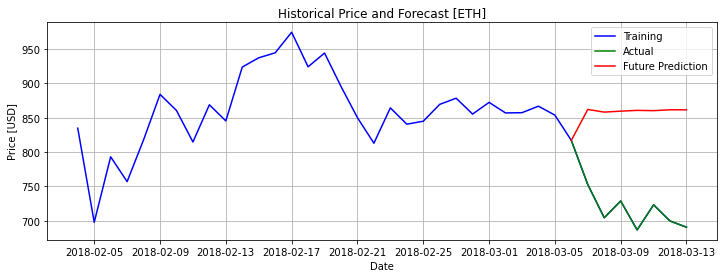
\includegraphics[width=0.5\textwidth]{./plots/arima/plots_eth_random_monthly/eth_mth4}} \\
   \subfloat[]{
   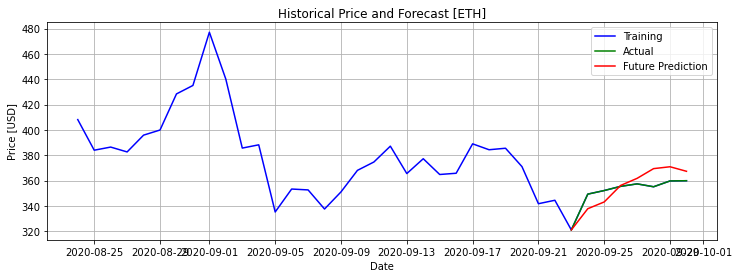
\includegraphics[width=0.5\textwidth]{./plots/arima/plots_eth_random_monthly/eth_mth5}}
   \subfloat[]{
   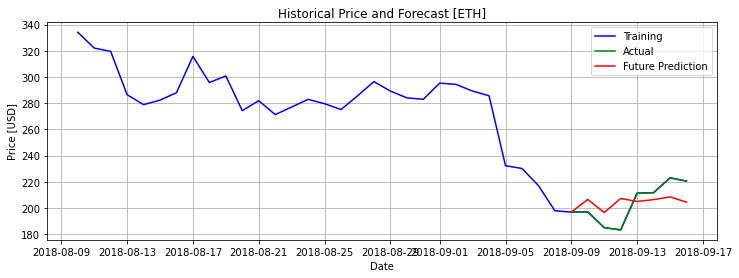
\includegraphics[width=0.5\textwidth]{./plots/arima/plots_eth_random_monthly/eth_mth6}} \\
   \subfloat[]{
   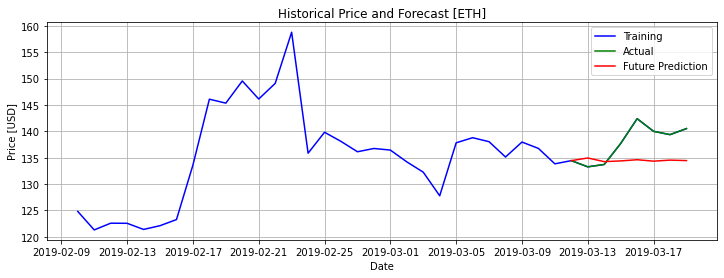
\includegraphics[width=0.5\textwidth]{./plots/arima/plots_eth_random_monthly/eth_mth7}}
   \subfloat[]{
   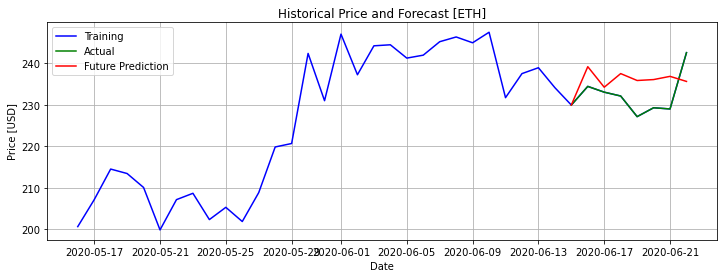
\includegraphics[width=0.5\textwidth]{./plots/arima/plots_eth_random_monthly/eth_mth8}} \\
   \subfloat[]{
   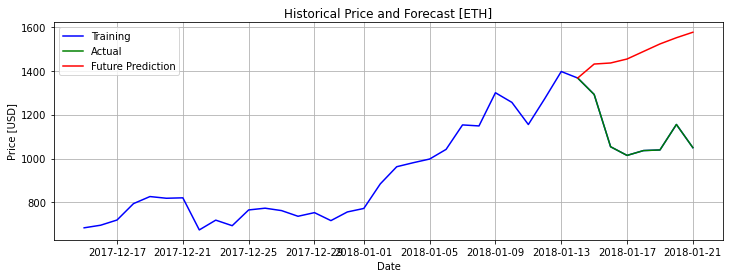
\includegraphics[width=0.5\textwidth]{./plots/arima/plots_eth_random_monthly/eth_mth9}}
   \subfloat[]{
   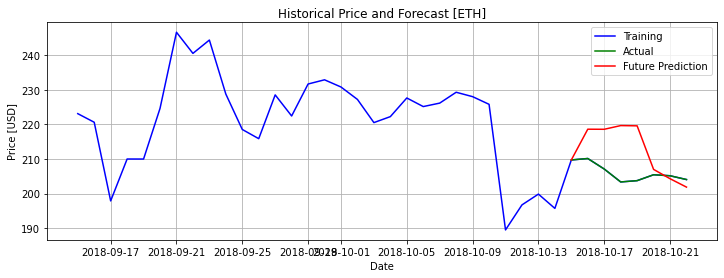
\includegraphics[width=0.5\textwidth]{./plots/arima/plots_eth_random_monthly/eth_mth10}}
  \caption{Predicción del modelo entrenado con 10 semanas aleatorias de ETH}
  \label{f:eth_mth_arima}
\end{figure}

\begin{table}[t]
 \begin{center}
  \begin{tabular}{|r|c|c|c|c|c|c|c|c|c|c|}
    Métrica & (a) & (b) & (c) & (d) & (e) & (f) & (g) & (h) & (i) & (j) \\ \hline
    MAE &  &  &  &  &  &  &  &  &  &  \\
    RMSE &  &  &  &  &  &  &  &  &  & \\
    sMAPE &  &  &  &  &  &  &  &  &  & \\ \hline
  \end{tabular}
  \caption{Fruta disponible}
  \label{tab:eth}
 \end{center}
\end{table}

\begin{figure}
 \centering
  \subfloat[]{
   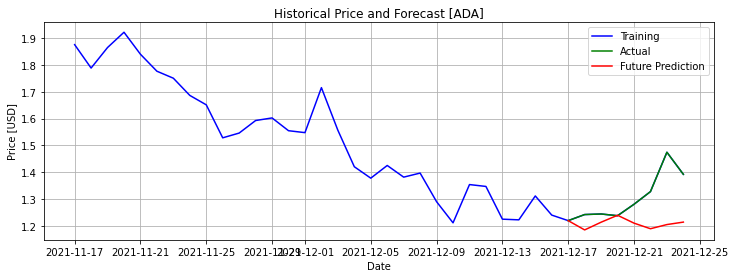
\includegraphics[width=0.5\textwidth]{./plots/arima/plots_ada_random_monthly/ada_mth1}}
  \subfloat[]{
   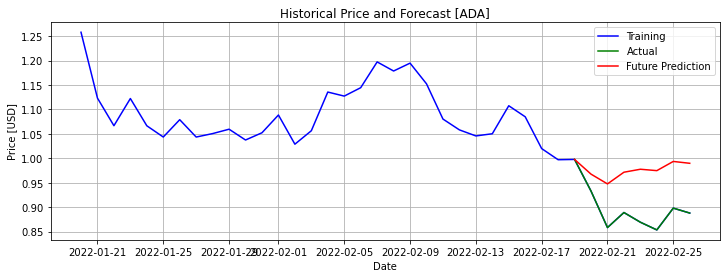
\includegraphics[width=0.5\textwidth]{./plots/arima/plots_ada_random_monthly/ada_mth2}} \\
  \subfloat[]{
   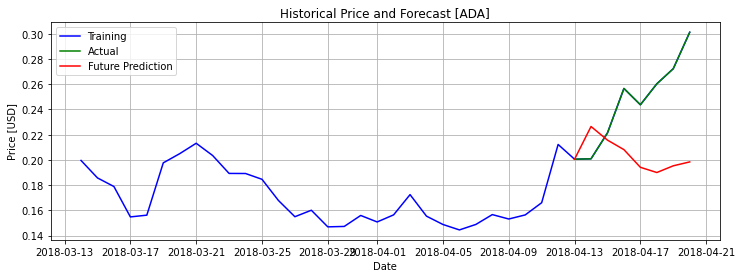
\includegraphics[width=0.5\textwidth]{./plots/arima/plots_ada_random_monthly/ada_mth3}}
   \subfloat[]{
   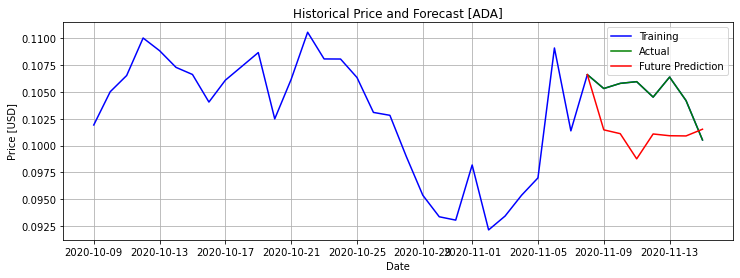
\includegraphics[width=0.5\textwidth]{./plots/arima/plots_ada_random_monthly/ada_mth4}} \\
   \subfloat[]{
   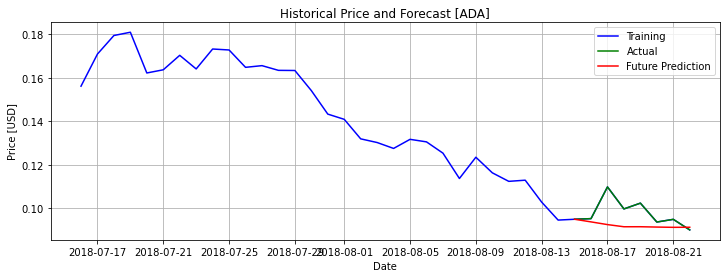
\includegraphics[width=0.5\textwidth]{./plots/arima/plots_ada_random_monthly/ada_mth5}}
   \subfloat[]{
   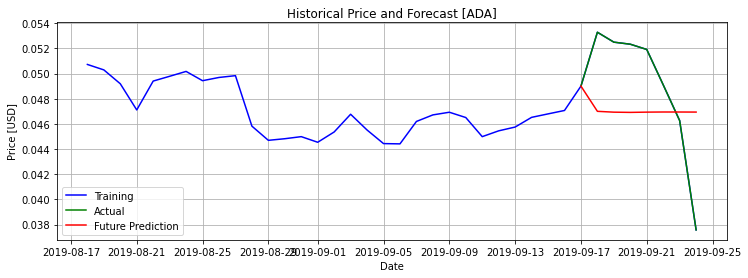
\includegraphics[width=0.5\textwidth]{./plots/arima/plots_ada_random_monthly/ada_mth6}} \\
   \subfloat[]{
   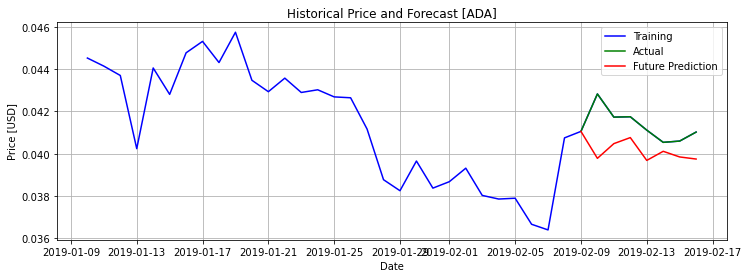
\includegraphics[width=0.5\textwidth]{./plots/arima/plots_ada_random_monthly/ada_mth7}}
   \subfloat[]{
   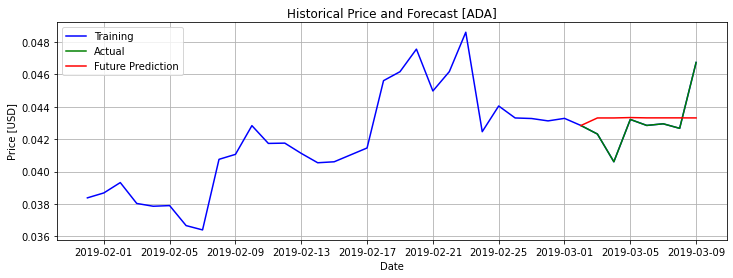
\includegraphics[width=0.5\textwidth]{./plots/arima/plots_ada_random_monthly/ada_mth8}} \\
   \subfloat[]{
   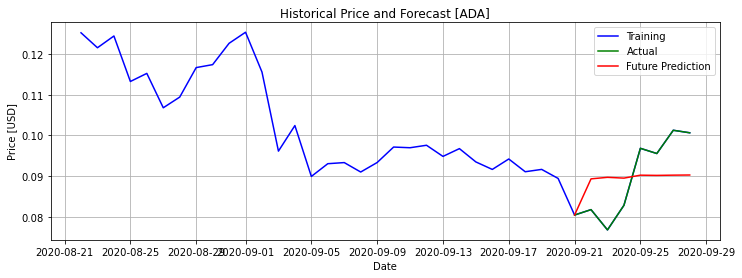
\includegraphics[width=0.5\textwidth]{./plots/arima/plots_ada_random_monthly/ada_mth9}}
   \subfloat[]{
   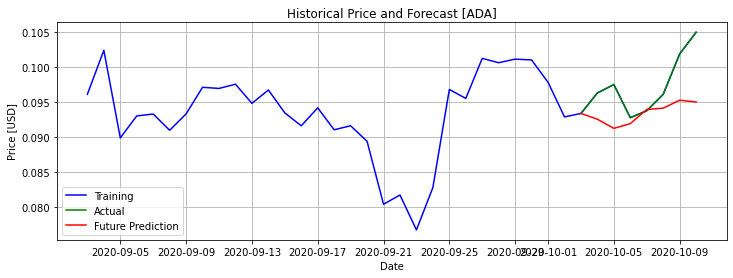
\includegraphics[width=0.5\textwidth]{./plots/arima/plots_ada_random_monthly/ada_mth10}}
  \caption{Predicción del modelo entrenado con 10 semanas aleatorias de ADA}
  \label{f:ada_mth_arima}
\end{figure}

\begin{table}[t]
 \begin{center}
  \begin{tabular}{|r|c|c|c|c|c|c|c|c|c|c|}
    Métrica & (a) & (b) & (c) & (d) & (e) & (f) & (g) & (h) & (i) & (j) \\ \hline
    MAE &  &  &  &  &  &  &  &  &  &  \\
    RMSE &  &  &  &  &  &  &  &  &  & \\
    sMAPE &  &  &  &  &  &  &  &  &  & \\ \hline
  \end{tabular}
  \caption{Fruta disponible}
  \label{tab:ada}
 \end{center}
\end{table}

\end{document}
